\chapter{电磁感应}

本章讨论法拉第电磁感应定律、楞次定律、自感、互感以及由机械运动与电路耦合形成的动力学问题。基本关系为
\[
\mathcal{E}=-\dv{\Phi}{t},
\qquad
\Phi=\int \vb*{B}\cdot \dd{\vb*{S}}.
\]

\begin{classic}
两条光滑平行金属导轨间距为 $l$，导轨所在平面与匀强磁场垂直，磁感应强度为 $B$。一根金属棒以速度 $v$ 沿导轨匀速运动，电路总电阻为 $R$。求：
\begin{enumerate}
  \item 感应电动势；
  \item 回路电流；
  \item 金属棒所受安培力大小，并说明外力做功与电路发热的关系。
\end{enumerate}

\begin{center}
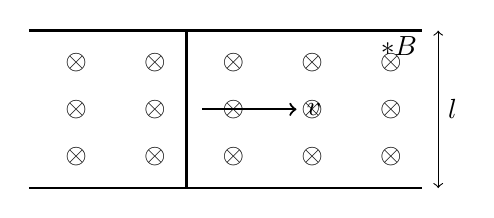
\begin{tikzpicture}[scale=1.0]
  \draw[thick] (0,0) -- (5,0);
  \draw[thick] (0,2) -- (5,2);
  \draw[very thick] (2,0) -- (2,2);
  \draw[->,thick] (2.2,1) -- (3.4,1) node[right] {$v$};
  \foreach \x in {0.6,1.6,2.6,3.6,4.6}
    \foreach \y in {0.4,1.0,1.6}
      \node at (\x,\y) {$\otimes$};
  \node at (4.7,1.8) {$\vb*{B}$};
  \draw[<->] (5.2,0) -- (5.2,2) node[midway,right] {$l$};
\end{tikzpicture}
\end{center}

\begin{solution}
切割磁感线产生的感应电动势为
\[
\mathcal{E}=Blv.
\]
回路电流
\[
I=\frac{\mathcal{E}}{R}=\frac{Blv}{R}.
\]
金属棒受安培力
\[
F=BIl=B\cdot \frac{Blv}{R}\cdot l=\frac{B^2l^2v}{R}.
\]
若金属棒做匀速运动，则外力应与安培力平衡。外力功率
\[
P_{\text{外}}=Fv=\frac{B^2l^2v^2}{R}.
\]
而电路发热功率
\[
P_{\text{热}}=I^2R=\qty(\frac{Blv}{R})^2R=\frac{B^2l^2v^2}{R}.
\]
二者相等，表明外界输入的机械功率全部转化为电路中的焦耳热。
\end{solution}
\end{classic}

\begin{classic}
一匝数为 $N$、面积为 $S$ 的线圈放在匀强磁场中，线圈平面法线与磁场夹角为 $\theta$。若磁感应强度随时间变化为 $B(t)=B_0+kt$，求线圈中的感应电动势，并讨论以下两种情况：
\begin{enumerate}
  \item 线圈静止；
  \item $B$ 不变而线圈匀速转动，$\theta=\omega t$。
\end{enumerate}

\begin{solution}
磁通量为
\[
\Phi=NB S\cos\theta.
\]
当线圈静止时，$\theta$ 不变，而 $B=B_0+kt$，故
\[
\mathcal{E}=-\dv{\Phi}{t}=-NS\cos\theta\dv{B}{t}=-NSk\cos\theta.
\]
感应电动势大小为
\[
|\mathcal{E}|=NSk|\cos\theta|.
\]
若 $B$ 不变而线圈以角速度 $\omega$ 匀速转动，$\theta=\omega t$，则
\[
\Phi=NBS\cos \omega t,
\]
故
\[
\mathcal{E}=-\dv{\Phi}{t}=NBS\omega\sin\omega t.
\]
这说明感应电动势既可以由“磁场大小变化”产生，也可以由“线圈取向变化”产生，本质上都源于磁通量随时间改变。
\end{solution}
\end{classic}

\begin{classic}
一自感系数为 $L$ 的线圈中电流由 $0$ 均匀增大到 $I_0$，所经历时间为 $T$。请从微积分角度求自感电动势，并进一步求外界在建立该电流过程中向磁场储存的能量。

\begin{solution}
电流变化率为
\[
\dv{i}{t}=\frac{I_0}{T}.
\]
因此自感电动势
\[
\mathcal{E}_L=-L\dv{i}{t}=-L\frac{I_0}{T}.
\]
若某时刻电流为 $i$，再增加微元 $\dd{i}$，外界克服反电动势做功
\[
\dd{W}=L i\,\dd{i}.
\]
于是总储能
\[
W=\int_0^{I_0} Li\,\dd{i}=\frac12 LI_0^2.
\]
这个推导与电容器储能完全类似：前者把能量存于磁场，后者把能量存于电场。
\end{solution}
\end{classic}

\begin{competition}
金属棒质量为 $m$，置于间距为 $l$ 的光滑导轨上，回路总电阻为 $R$，垂直轨道平面有匀强磁场 $B$。若棒在恒力 $F$ 作用下由静止开始运动，建立棒速率 $v(t)$ 的微分方程，并求稳态速度。

\begin{solution}
棒运动时产生感应电动势
\[
\mathcal{E}=Blv,
\qquad I=\frac{Blv}{R}.
\]
安培力大小
\[
F_m=BIl=\frac{B^2l^2}{R}v.
\]
由牛顿第二定律
\[
m\dv{v}{t}=F-\frac{B^2l^2}{R}v.
\]
这就是机械与电磁耦合得到的一阶微分方程。解得
\[
v(t)=\frac{FR}{B^2l^2}\qty(1-e^{-\frac{B^2l^2}{mR}t}).
\]
因此稳态速度为
\[
v_{\infty}=\frac{FR}{B^2l^2}.
\]
当速度增大时，感应电流与安培阻力随之增大，最终与外力平衡，这是一类典型的“磁阻尼”过程。
\end{solution}
\end{competition}

\begin{competition}
在整块金属板穿过磁场边界时会产生涡流。请做一个定量近似分析：若可把涡流简化成等效电阻为 $R_e$ 的闭合回路，磁通量近似以速率 $\dv{\Phi}{t}=\alpha v$ 变化，其中 $v$ 为金属板速度，$\alpha$ 为几何常量，求磁制动力与速度的关系，并说明其阻尼本质。

\begin{solution}
感应电动势大小为
\[
\mathcal{E}=\alpha v.
\]
于是涡流电流
\[
I=\frac{\alpha v}{R_e}.
\]
感应电流与外磁场相互作用会产生反向阻力。若把等效磁制动力写成与电流成正比、且比例系数为另一几何磁学常量 $\beta$，则
\[
F_d=\beta I=\frac{\alpha\beta}{R_e}v.
\]
因此在该近似下，磁制动力与速度成正比，即
\[
F_d=kv.
\]
其本质是：运动越快，磁通变化越快，感应电流越大，依据楞次定律形成的反向力也越强，从而把机械能持续转化为焦耳热。这正是电磁刹车系统广泛应用的物理基础。
\end{solution}
\end{competition}

\begin{competition}
两线圈靠近放置，互感系数为 $M$。若线圈 1 中电流为 $i_1(t)=I_0\sin\omega t$，求线圈 2 中由互感产生的感应电动势，并说明互感电压相位与原电流的关系。

\begin{solution}
线圈 2 中由线圈 1 产生的磁通量与 $i_1$ 成正比，可写为
\[
\Phi_{21}=Mi_1.
\]
故感应电动势
\[
\mathcal{E}_2=-\dv{\Phi_{21}}{t}=-M\dv{i_1}{t}=-M\omega I_0\cos\omega t.
\]
也可写成
\[
\mathcal{E}_2=M\omega I_0\sin\qty(\omega t-\frac{\pi}{2}).
\]
因此互感电压相对于原电流超前或滞后四分之一个周期的表述取决于采用正弦还是余弦基准；本质上它与原电流的时间导数同相。这与自感电压 $\mathcal{E}_L=-L\dv*{i}{t}$ 具有完全类似的数学结构。
\end{solution}
\end{competition}

\begin{university}
交流发电机的单匝线圈面积为 $S$，在匀强磁场 $B$ 中以角速度 $\omega$ 匀速转动，转轴垂直于磁场。请完整写出磁通量、感应电动势以及外接纯电阻 $R$ 时的电流表达式。

\begin{center}
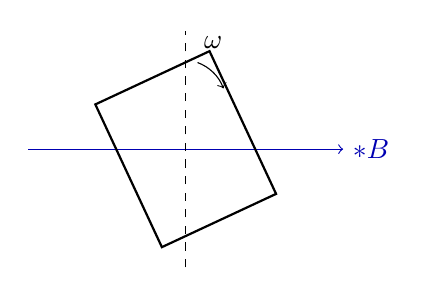
\begin{tikzpicture}[scale=1.0]
  \draw[->,blue!70!black] (-2,0) -- (2,0) node[right] {$\vb*{B}$};
  \draw[thick,rotate=25] (-0.8,-1.0) rectangle (0.8,1.0);
  \draw[dashed] (0,-1.5) -- (0,1.5);
  \node at (0.35,1.35) {$\omega$};
  \draw[->] (0.15,1.1) arc (70:20:0.55);
\end{tikzpicture}
\end{center}

\begin{solution}
设线圈法线与磁场夹角为
\[
\theta=\omega t.
\]
则磁通量
\[
\Phi=BS\cos\omega t.
\]
感应电动势
\[
\mathcal{E}=-\dv{\Phi}{t}=BS\omega\sin\omega t.
\]
若线圈有 $N$ 匝，则振幅应乘以 $N$。外接纯电阻 $R$ 时，电流为
\[
i(t)=\frac{\mathcal{E}}{R}=\frac{BS\omega}{R}\sin\omega t.
\]
其有效值分别为
\[
\mathcal{E}_{\text{rms}}=\frac{BS\omega}{\sqrt{2}},
\qquad
I_{\text{rms}}=\frac{BS\omega}{\sqrt{2}R}.
\]
这就是最基本的正弦交流发电模型。
\end{solution}
\end{university}

\begin{university}
质量为 $m$ 的导体板进入磁场区域后受到与速度成正比的磁阻尼力 $F_d=-kv$。若初速度为 $v_0$，求速度和位移随时间的关系，并说明为什么常称其为“指数衰减磁制动”。

\begin{solution}
由牛顿第二定律
\[
m\dv{v}{t}=-kv.
\]
分离变量积分得
\[
\frac{\dd{v}}{v}=-\frac{k}{m}\dd{t}
\Rightarrow v(t)=v_0e^{-kt/m}.
\]
再积分求位移（以 $x(0)=0$ 为初值）：
\[
x(t)=\int_0^t v_0e^{-k\tau/m}\dd{\tau}
=\frac{mv_0}{k}\qty(1-e^{-kt/m}).
\]
由于速度按指数函数衰减，所以称为指数衰减磁制动。它反映了当阻力正比于速度时，系统不会在有限时间内完全停下，而是渐近趋于静止。
\end{solution}
\end{university}

\begin{university}
在 RL 串联电路中，电流建立过程中电源提供的能量如何分配到电阻发热与电感储能中？请给出定性与定量说明。

\begin{solution}
RL 串联电路满足
\[
L\dv{i}{t}+Ri=\mathcal{E}.
\]
随着电流从 $0$ 建立到稳态 $I_\infty=\mathcal{E}/R$，电源持续输出能量。其一部分通过
\[
P_R=i^2R
\]
转化为焦耳热，另一部分通过
\[
P_L=u_L i=L i\dv{i}{t}
\]
储存在磁场中。

若只看最终储能，则当电流达到某一瞬时值 $i$ 时，电感中磁场能为
\[
W_L=\int_0^i Li\,\dd{i}=\frac12 Li^2.
\]
在建立过程中，电阻发热是不可逆耗散，而电感储能是可逆储存；断电时，电感又可以通过自感把这部分磁场能释放出来。这种能量分配正是电感“阻碍电流变化”但又“不消耗能量”的根本原因。
\end{solution}
\end{university}

\begin{problem}
请从感应电流与磁场相互作用的角度，定性分析电磁悬浮的可能机制，并解释为什么稳定悬浮通常需要动态控制、旋转体或特殊材料（如超导体）。

\begin{solution}
导体或磁性体处在变化磁场中时，会产生感应电流或磁化效应。依据楞次定律，这些响应倾向于阻碍相对运动或磁通变化，因此有可能形成向上的电磁力，实现“悬浮”。例如高速变化磁场可在导体中激发涡流，涡流与外磁场相互作用产生排斥力。

但单靠静态经典磁场很难实现对普通物体的稳定三维悬浮，这与 Earnshaw 定理有关。因此工程上往往需要：
\begin{enumerate}
  \item 主动反馈控制，实时调节电流维持平衡；
  \item 借助旋转陀螺效应提高稳定性；
  \item 利用超导体的完全抗磁性与磁通钉扎获得稳定约束。
\end{enumerate}
因此电磁悬浮不仅是力学平衡问题，更是稳定性问题。
\end{solution}
\end{problem}

\begin{problem}
感应加热广泛用于金属熔炼与表面淬火。请定性说明其工作原理，并讨论频率选择、集肤效应和材料电阻率对加热效果的影响。

\begin{solution}
感应加热利用交变电流在线圈周围产生交变磁场，使工件内部出现感应电动势和涡流。涡流在材料电阻作用下产生焦耳热，从而实现无接触加热。若材料具有磁性，还可能伴随磁滞损耗，共同提高发热效率。

频率越高，磁场变化越快，感应电动势通常越大，但电流更集中于材料表层，即集肤效应增强，因此适合表面加热与淬火；频率较低则更有利于深层加热。材料电阻率过低时不易发热，过高时电流又难以充分流动，因此实际工艺需综合考虑频率、线圈结构、材料磁导率与电阻率，以获得理想的加热深度和效率。
\end{solution}
\end{problem}
